  %%%%%%%%%%%%%%%%%%%%%%%%%%%%%%%%%%%%%%%%%%
  %%                                      %%
  %%AQUI SÃO INSERIDOS OS PACOTES DO LATEX%%
  %%                                      %%
  %%%%%%%%%%%%%%%%%%%%%%%%%%%%%%%%%%%%%%%%%%
  
\documentclass[a4paper, 12pt]{article}
\usepackage[top=3cm, botton=2cm, left=3cm, right=2cm]{geometry}
\usepackage[utf8]{inputenc}
\usepackage{float}
\usepackage{graphicx}
\usepackage[brazilian, english]{babel}
\usepackage{fancyhdr}
\usepackage{amsmath, amsfonts, amssymb}ex

\usepackage{epigraph}
\usepackage{tabularx}
\usepackage{abstract}
\usepackage{subfig}

%%%%%%%%%%%%%%%%%%%%%%%%%%%%%%%%%%%%%%%%%%%%%%%%%%%%
%%  USADO PARA PRODUZIRMOS UMA CAPA PARA O ARTIGO %%
%%%%%%%%%%%%%%%%%%%%%%%%%%%%%%%%%%%%%%%%%%%%%%%%%%%%
                                               
%\documentclass{ufpethesis}
%\title{Aqui é o título}
%\author{Nome do autor}
%\date{2015}




%% INÍNCIO DO ARTIGO %%

\begin{document}

\graphicspath{{imagens/}{referencias/}{logo/}}  %% Referenciando subpastas no arquivo %%

%% ESPAÇO DIDICADO À AGRADECIMENTOS, RESUMO E ABSTRACT %%

\begin{titlepage}

\selectlanguage{brazilian}
\begin{abstract}
Texto em Português
\end{abstract}
\begin{footnotesize}
\textbf{Palavras-chave:} \textit{Palavras-chave}
\end{footnotesize}
\newpage

\end{titlepage}

\begin{titlepage}

\selectlanguage{english}
\begin{abstract}
 Text in English
\end{abstract}
\begin{footnotesize}
\textbf{keywords:} \textit{key words}
\end{footnotesize}
\newpage

%\begin{center}
%\textbf{Agradecimentos}
%\end{center}

%Agradecimentos aqui!

\end{titlepage}

%% EPÍGRAFE DO ARTIGO %%
\begin{titlepage}

   \epigraph{\textit{"A caridade é o processo de somar alegrias, diminuir males, multiplicar esperanças e dividir a felicidade para que a Terra se realize na condição do esperado Reino de Deus."}}{Emmanuel} \newpage

\end{titlepage}
\newpage



%%  SUMÁRIO  %%
\selectlanguage{brazilian}
\tableofcontents \newpage  %% ESTE COMANDO ABILITA O SUMÁRIO NO ARTIGO  %% 

%%  LISTA DE FIGURAS E TABELAS %%

\listoffigures
%\listoftables
\newpage

%  Comando para a insersão da capa neste ponto do artigo  $$
%\maketitle

%% LOGOTIPO NO CABEÇALHO %%
\pagestyle{fancy} \newpage
\lhead{
\includegraphics[width=1cm]{logo_anhanguera}}

%% NOTAS DE RODAPÉ %%
\rfoot{\begin{small}Roda pé \end{small}}
\lfoot{}



%%%%%%%%%%%%%%%%%%%%%%%%%%%%%%%%%%
%%%                            %%%
%%% INÍCIO DO CORPO DO ARTIGO, %%%
%%%                            %%%
%%%%%%%%%%%%%%%%%%%%%%%%%%%%%%%%%%


\section{IMAGENS}

%% Inclusão de Figuras %%


%% inclusão de SubFiguras %%

\begin{figure}[!htb]
\centering
\subfloat[Aline]{

\includegraphics[height=4cm]{1}
\label{figdroopy}
}
\quad %espaco separador
\subfloat[Mel]{

\includegraphics[height=4cm]{2}
\label{figsnoop}
}
\caption{Minhas Vidas}
\label{fig01}
\end{figure}

\begin{figure}[!htb]
\centering
\subfloat[Aline]{

\includegraphics[height=4cm]{3}
\label{figdroopy}
}
\quad %espaco separador
\subfloat[Mel]{
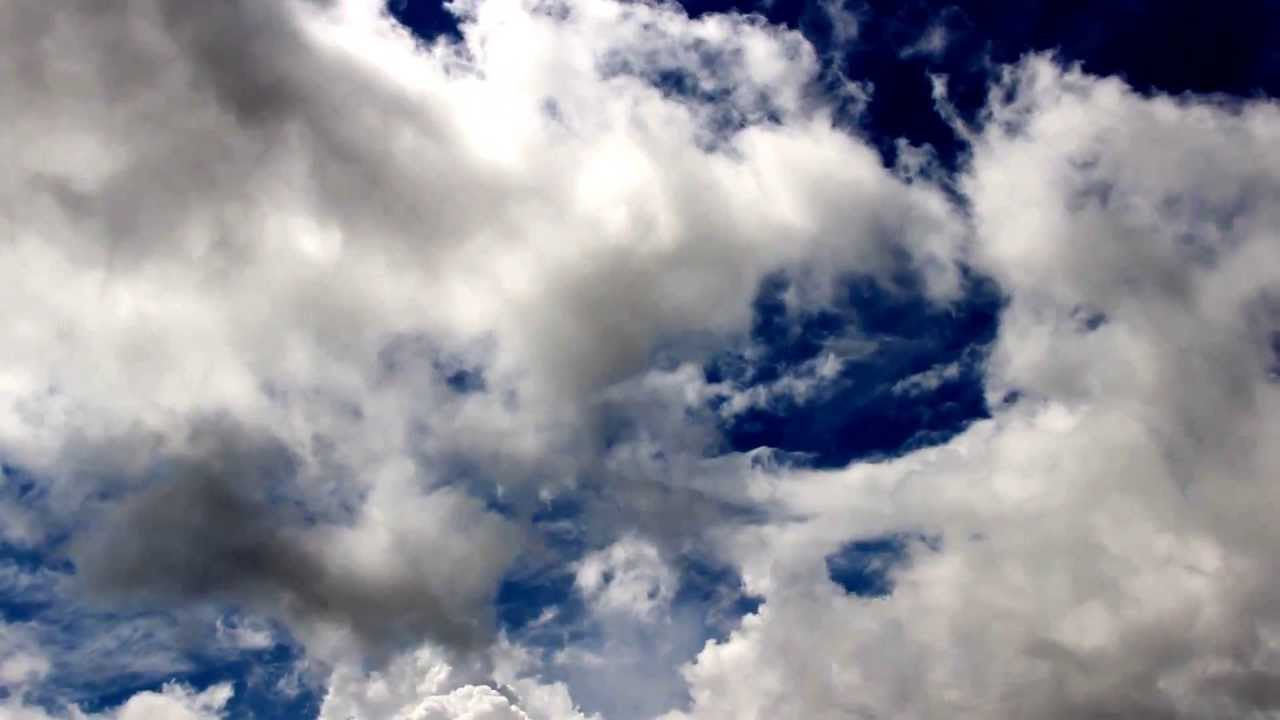
\includegraphics[height=4cm]{4}
\label{figsnoop}
}
\caption{Minhas Vidas}
\label{fig01}
\end{figure}


\begin{figure}[!htb]
\centering
\subfloat[Aline]{
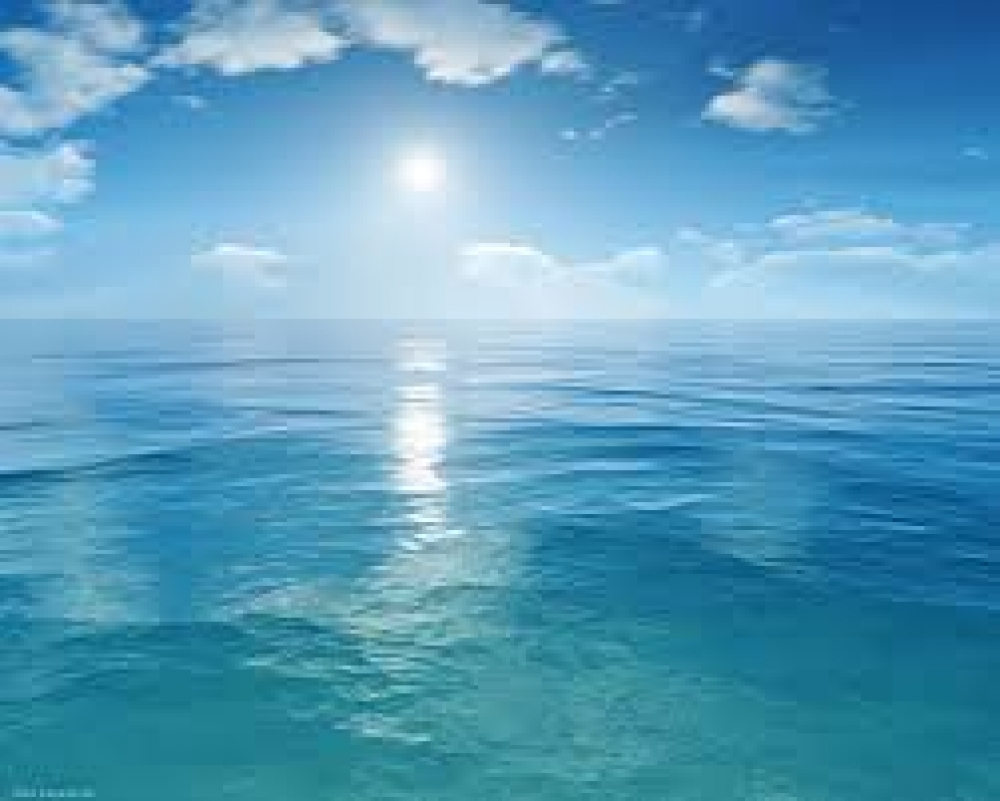
\includegraphics[height=4cm]{5}
\label{figdroopy}
}
\quad %espaco separador
\subfloat[Mel]{
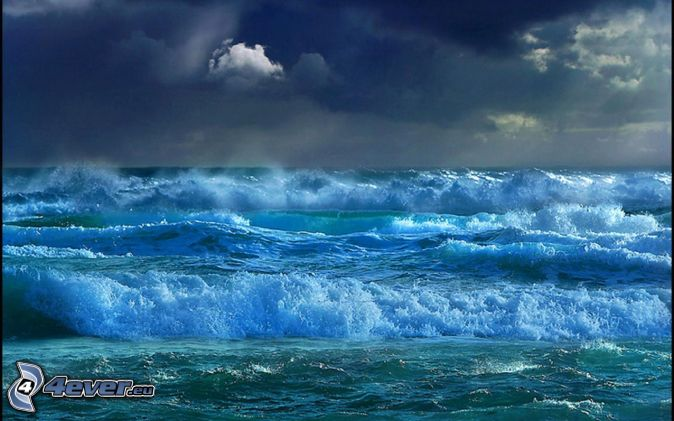
\includegraphics[height=4cm]{6}
\label{figsnoop}
}
\caption{Minhas Vidas}
\label{fig01}
\end{figure}



\begin{figure}[!htb]
\centering
\subfloat[Aline]{
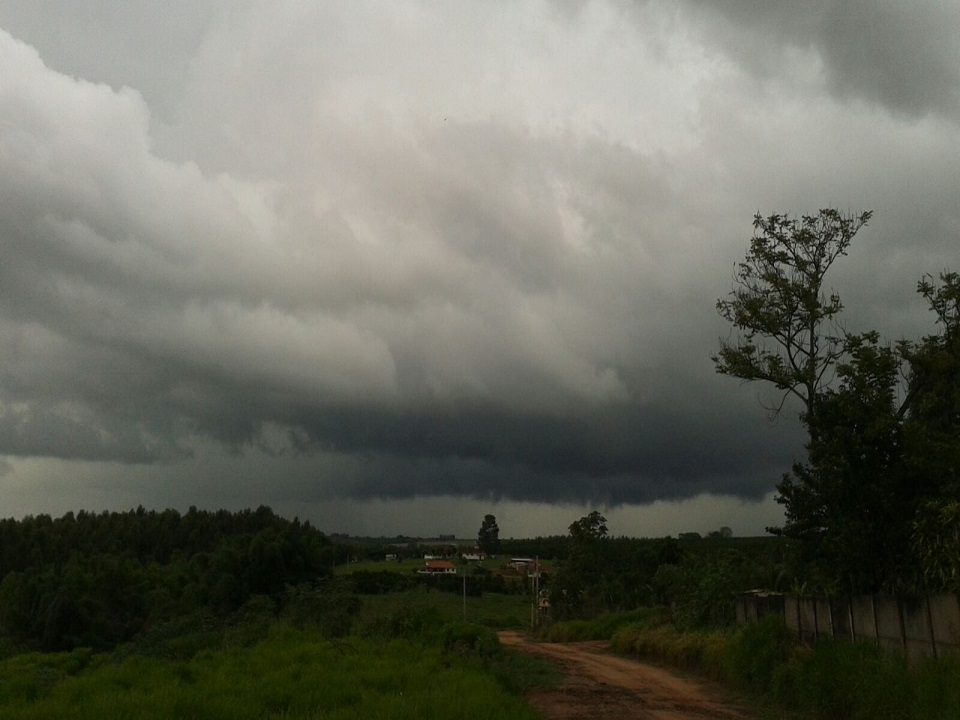
\includegraphics[height=4cm]{7}
\label{figdroopy}
}
\quad %espaco separador
\subfloat[Mel]{
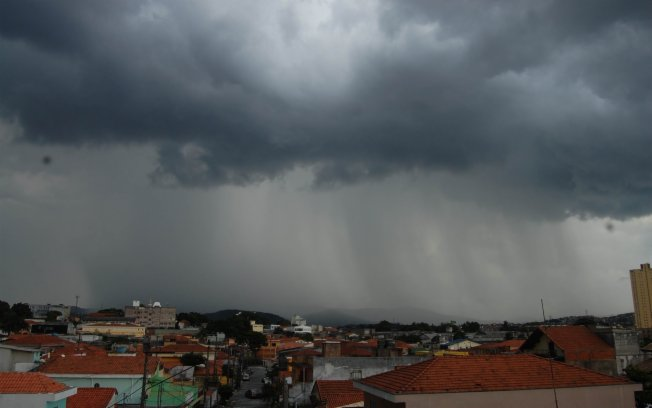
\includegraphics[height=4cm]{8}
\label{figsnoop}
}
\caption{Minhas Vidas}
\label{fig01}
\end{figure}

\begin{figure}[!htb]
\centering
\subfloat[Aline]{
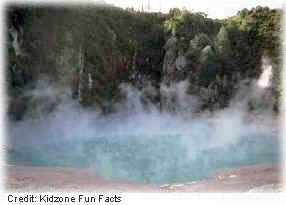
\includegraphics[height=4cm]{9}
\label{figdroopy}
}
\quad %espaco separador
\subfloat[Mel]{

\includegraphics[height=4cm]{1}
\label{figsnoop}
}
\caption{Minhas Vidas}
\label{fig01}
\end{figure}






 

%%% REFERENCIAS BIBLIOGRAFICAS %% 
\newpage
\bibliographystyle{plain}
\addcontentsline{toc}{section}{REFERÊNCIAS} 
\bibliography{referencias/biblio.bib}

\cite{evangelho}
\cite{le}


\end{document}
